\subsubsection{Design}
Da SharedLib blev udarbejdet, var der stort fokus på SOLID's designprincipper, da disse muliggjorde den ønskede funktionalitet, hvis disse blev overholdt. Dette betød at protokollen specielt blev bygget op omkring tre hovedbegreber:

\begin{itemize}
	\item \textbf{Models}
	\item \textbf{Commands} 
	\item \textbf{Marshallers}
\end{itemize}

\textbf{Models}\\
Også omtalt som datamodeller indeholder blot attributter med relevant data og bliver brugt som domæneklasser.\\\\
\textbf{Command}\\
Kommandoer som "send produktkataloget" og "Opret produkt" blev skabt som højniveau Command klasser der kunne tage relevant data eller eventuelt datamodeller som parametre. \\\\
\textbf{Marshaller}\\
De klasser der skulle omdanne en specifik kommando til en tilsvarende XML string og samtidigt kunne afkode en XML string og gengive denne i et korrekt kommando objekt.\\


Modeller indeholder som udgangspunkt forskellige ønskede data og bliver som oftest brugt i forbindelse med kommandoer. Dette betyder at hvis der bliver oprettet en "opret produkt" kommando, så kan der gives en Product datamodel i constructoren så kommandoen altså indeholder nøjagtigt disse attributter. 

Commands bliver herefter brugt som enten et parameter i en Encode funktion (se figur \ref{fig:EncodeSL}) eller bliver returneret fra en Decode funktion (se figur \ref{fig:DecodeSL}). 

Disse funktionskald bliver håndteret af en marshaller, specifik for den kommando der er sendt med som parameter. Selve marshalleren sørger for at lave Encode, som skaber og returnerer XML ud fra objektet, eller Decode, som skaber og returnerer et objekt ud fra en string med XML.

\begin{figure}[H]
	\centering
	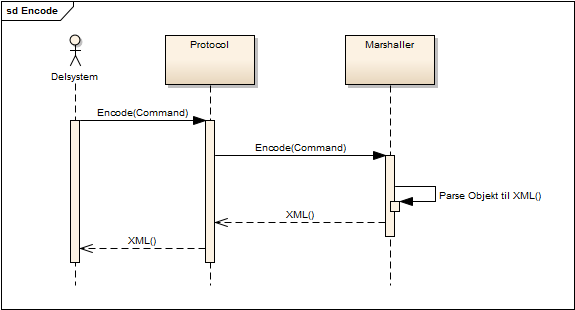
\includegraphics[width=0.8\textwidth]{Projektbeskrivelse/DesignOgImplementering/SharedLib/Images/Rapport/Encode.png}
	\caption{Overordnet sekvensdiagram over encode funktionen}
	\label{fig:EncodeSL}
\end{figure}

\begin{figure}[H]
	\centering
	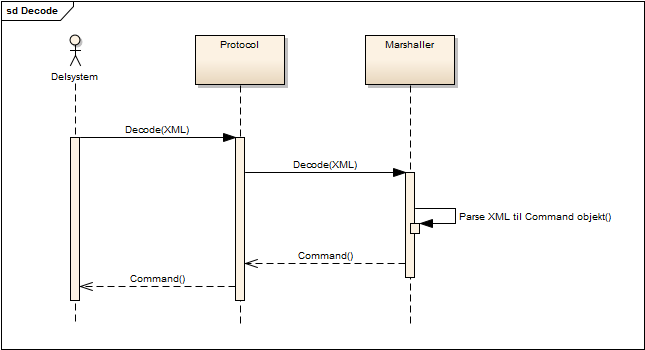
\includegraphics[width=0.8\textwidth]{Projektbeskrivelse/DesignOgImplementering/SharedLib/Images/Rapport/Decode.png}
	\caption{Overordnet sekvensdiagram over decode funktionen}
	\label{fig:DecodeSL}
\end{figure}

Med disse begreber på plads kunne SOLID's designprincipper pludseligt defineres klart i forhold til protokollen:\\

\textbf{S}, Single Responsibility, blev overholdt i og med hver enkelt kommando ville få sin egen klasse, der skulle håndtere denne. Denne kommando ville samtidig have sin egen specifikke marshaller, hvis eneste formål var at parse netop den type af kommando.\\

\textbf{O}, Open-Closed princippet, blev også overholdt da alle kommandoer og alle marshallers hver havde implementeret hver deres interface. Dette betyder at hvis en ny kommando skal tilføjes skal den nye kommando blot implementere den abstrakte klasse Command og derefter skal der oprettes en marshallers der implementerer marshaller interfacet, og på den måde vil en ny kommando ikke have nogen indflydelse på den allerede eksisterende kode.\\

\textbf{L}, Liskov's substitutions princip, fortæller at en superklasse skal kunne byttes ud med dens subklasse uden at dette ændre funktionaliteten i programmet. Dette havde ikke den store indflydelse på protokollen da der kun blev nedarvet fra Command klassen og da denne kun indeholder attributter blev der ikke brudt med dette princip.\\

\textbf{I}, Interface segregation, dette princip betyder at hvis der ønskes en specifik funktion i et større system, bør der så vidt muligt være interfaces der sørger for at den ønskede funktionalitet kan tilgås uden at være tvunget til at tage stilling til og håndtere unødvendige funktioner. Dette blev også opnået og grundigt gennemtænkt i protokollen da der er blevet oprettet interfaces for alle klasser, single responsibility går dog lidt i hånd med dette punkt, da det på grund af dette princip er meget let at tilgå den ønskede funktionalitet, uden at skulle håndtere unødvendig funktionalitet.\\

\textbf{D}, Dependency inversion, kræver at afhængigheder skal komme nede fra og op. Ment som at en superklasse ikke skal kende til klasser i lavere lag på trods af at den måske bruger dem aktivt, dette skal fungerer via et interface i samme lag, som så bliver implementeret af en klasse i et lavere lag der her udfører disse handlinger. Dette er også indført i protokollen med de mange interfaces der f.eks. gør at protokol klassen ikke kender til de specifikke marshallers på trods af de bliver brugt når denne kalder encode funktionen på et marshaller interface. \\ 